\chapter{Muons in ATLAS}
  
\textit{I really need to find a quote for this chapter}
\vspace{5mm}
\begin{flushright}
--- Miha Zgubi\v{c}
\end{flushright}

\thispagestyle{empty}
\newpage
The ATLAS detector, described in the previous chapter, is a monument
to the engineers and physicists who designed and built it. However,
in order to turn its raw output of nearly one hundred million readout
channels per event to physics knowledge, it requires an intermediate step:
the reconstruction of physics objects.

Muons, the central physics object in this thesis, are reconstructed
by combining the information from the tracker and the muon spectrometer.
In order to be able to do precision studies the Monte Carlo (MC)
simulation of the detector response needs to be calibrated to match
the response in the real detector. In particular, the transverse momentum of
muons needs to be calibrated to the resolution obtained in the real
detector. Similarly, the reconstruction, track-to-vertex-association (TTVA),
and isolation efficiencies need to be calibrated to match those in 
recorded data. These calibrations are obtained through measurements
and carry associated uncertainties.

This chapter describes the first novel contributions from the author.
The first is an improved method of background subtraction in the isolation
efficiency measurements, which significantly reduces the systematic
uncertainty for muons with $\pt < 15$ \GeV. The second is an attempt
to improve muon momentum resolution.

\section{Reconstruction}

Tracks in the inner detector (ID) are reconstructed indiscriminately for
all charged particles. First, raw data from the detectors is converted
into space-points which form the basis of tracking. The main track finding
algorithm proceeds inside-out by finding the seeds in the silicon layers.
The seeds are then combined into roads and the extension to the TRT layer
is probed to add hits in the outermost layer. The final collection of hits
is fit to obtain the track parameters \cite{ATLAS-CONF-2010-072, Cornelissen:1020106}.
Tracks with at least $\pt > 400$ \MeV~and some other requirements, found
in Ref. \cite{ATL-PHYS-PUB-2015-026} are then used to find the primary
vertices. The reconstruction of primary vertices proceeds by first finding
the vertices and then fitting them \cite{Aaboud:2016rmg}. Finally, tracks
are associated with vertices which allows the computation of $d_0$, the
transverse impact parameter, which quantifies the shortest distance
between the track and the beam-line, and $z_0$, the longitudinal impact
parameter, which quantifies the difference between the $z$ coordinate
of the associated primary vertex, and the $z$ coordinate of the point
where $d_0$ is computed.

The reconstruction of tracks in the muon spectrometer (MS) proceeds by
first finding track segments in the MDT chambers using a Hough transform
\cite{ILLINGWORTH198887}, and then reconstructing them by fitting a
straight line to the associated hits. The segments are combined to
form MS tracks starting from the middle layer and finding compatible
segments in the inner and outer layers of the spectrometer. At least two
segments are needed to form a track, apart from the transition region
in which a single high quality segment can be used to build a track.
Finally, a global $\chi^2$ fit of the track is performed and the track
accepted if it satisfies the quality criteria. Otherwise, hits with 
high contribution to the $\chi^2$ value are removed and the track re-fit.
Hits can also be added to the track if they are consistent with the
track and the track is re-fit if these candidates are found \cite{Aad:2016jkr}.

Finally, the information from subdetectors is combined to form muon
candidates. Depending on which subdetectors are used for building the
candidate, four muon types are defined:
\begin{itemize}
\item Combined (CB) muons are reconstructed from a pair of tracks
in the ID and the MS. A global re-fit is performed using hits from 
both subdetectors with the flexibility to add or remove hits in the
MS to improve the fit quality. Most muons are reconstructed by the
outside-in approach extrapolating the MS tracks to the ID, but the
inside-out reconstruction is also used as the complementary approach 
\cite{Aad:2016jkr}.
\item Segment-tagged (ST) muons are formed by combining the ID track
with a single segment in the MDT or CSC chambers and were designed
to recover muon reconstruction efficiency for low $\pt$ muons which
only cross a single layer of the MS or cross the regions where
MS has poor acceptance \cite{Aad:2016jkr}.
\item Calorimeter-tagged (CT) muons match an ID track with a 
calorimeter deposit consistent with a minimum-ionising particle.
This type recovers the muon reconstruction efficiency in the regions
not covered by the MS, for example in the $|\eta|<0.1$, where cabling
and services to the ID are located, and where the support structure
is located. As a consequence of using the calorimeter this type has
the lowest purity \cite{Aad:2016jkr}.
\item Extrapolated (ME) muons are built from tracks in the MS that
are loosely compatible with originating from the interaction point.
This type is used to recover the reconstruction efficiency in the 
forward region $2.5 < |\eta| < 2.7$ not covered by the ID \cite{Aad:2016jkr}.
\end{itemize}
Finally, overlaps between different muons are resolved by order of
precedence starting with CB muons, followed by ST muons, and
finally the CT muons. ME ambiguities are resolved by analysing the
track fit quality and the number of hits.
The requirements on the number of hits and holes
\footnote{A \textit{hole} is an active sensor traversed by the
track that contains no hits. It also falls between two hits assigned to the track.}
in the ID and MS detectors are also used to guarantee a robust
measurement of $\pt$ \cite{Aad:2016jkr}.

In addition to that, a number of quality requirements must be
satisfied to differentiate between muons originating from the
interaction point (prompt muons) and the muons coming from the
decay of light hadrons. To this end the following variables are
defined for CB muons:
\begin{itemize}
\item normalised $\chi^2$ of the combined track fit.
\item $\rho' = \frac{|\pt^{\text{ID}} - \pt^{\text{MS}}|}{\pt^{\text{CB}}}$,
where the superscript denotes whether the $\pt$ refers to the
ID or MS muon candidate, or the CB muon.
\item $q/p$ significance $ = \frac{\left|\left(\frac{q}{p}\right)_\text{ID}
- \left(\frac{q}{p}\right)_\text{MS}\right|}
{\sqrt{\sigma^2_\text{ID} + \sigma^2_\text{MS}}}$,
where the $\left(\frac{q}{p}\right)$ is the measurement of the ratio of
the charge and the momentum, $\sigma$ are the uncertainties on
the corresponding quantities, and the subscript refers to whether
the measurement comes from the ID or the MS muon candidate.
\end{itemize}

Four overlapping muon identification selections, namely Loose, Medium, Tight,
and High-$\pt$, are supported by the muon performance group to 
serve different physics analyses and unify the evaluation of
systematic uncertainties arising from the selection requirements.
Tight muons maximise the purity of muons at the cost of some
identification efficiency and use only CB muons with additional
requirements on the track quality. Medium muons include CB and ME
muon types and are the default selection that minimises the systematic
uncertainties. Loose muons are designed to maximise the selection
efficiency and include all four muon types, with the CT and ST types
restricted to the $|\eta| < 0.1$ \cite{Aad:2016jkr}.

The fraction of prompt muons that are reconstructed and identified
is called reconstruction efficiency, and is in general different
in data and MC simulation. Efficiencies for Loose, Medium, and Tight
selections are shown in Figure \ref{fig:muon:reco_eff} for data and
MC simulation as a function of muon pseudorapidity. In the analysis,
MC simulation is corrected to data by applying weights, known as
scale factors, to account for the differences in efficiencies between
data and MC simulation. The scale factors are defined as
\begin{equation}
\text{SF} = \frac{\epsilon_\text{Data}}{\epsilon_\text{MC}},
\end{equation}
where SF is the scale factor, and $\epsilon$ is some efficiency,
as measured in data or MC simulation. The measurement of the
efficiencies, scale factors, and the associated
uncertainties is described in detail in Ref. \cite{Aad:2016jkr}.

\begin{figure}[h]
  \centering
  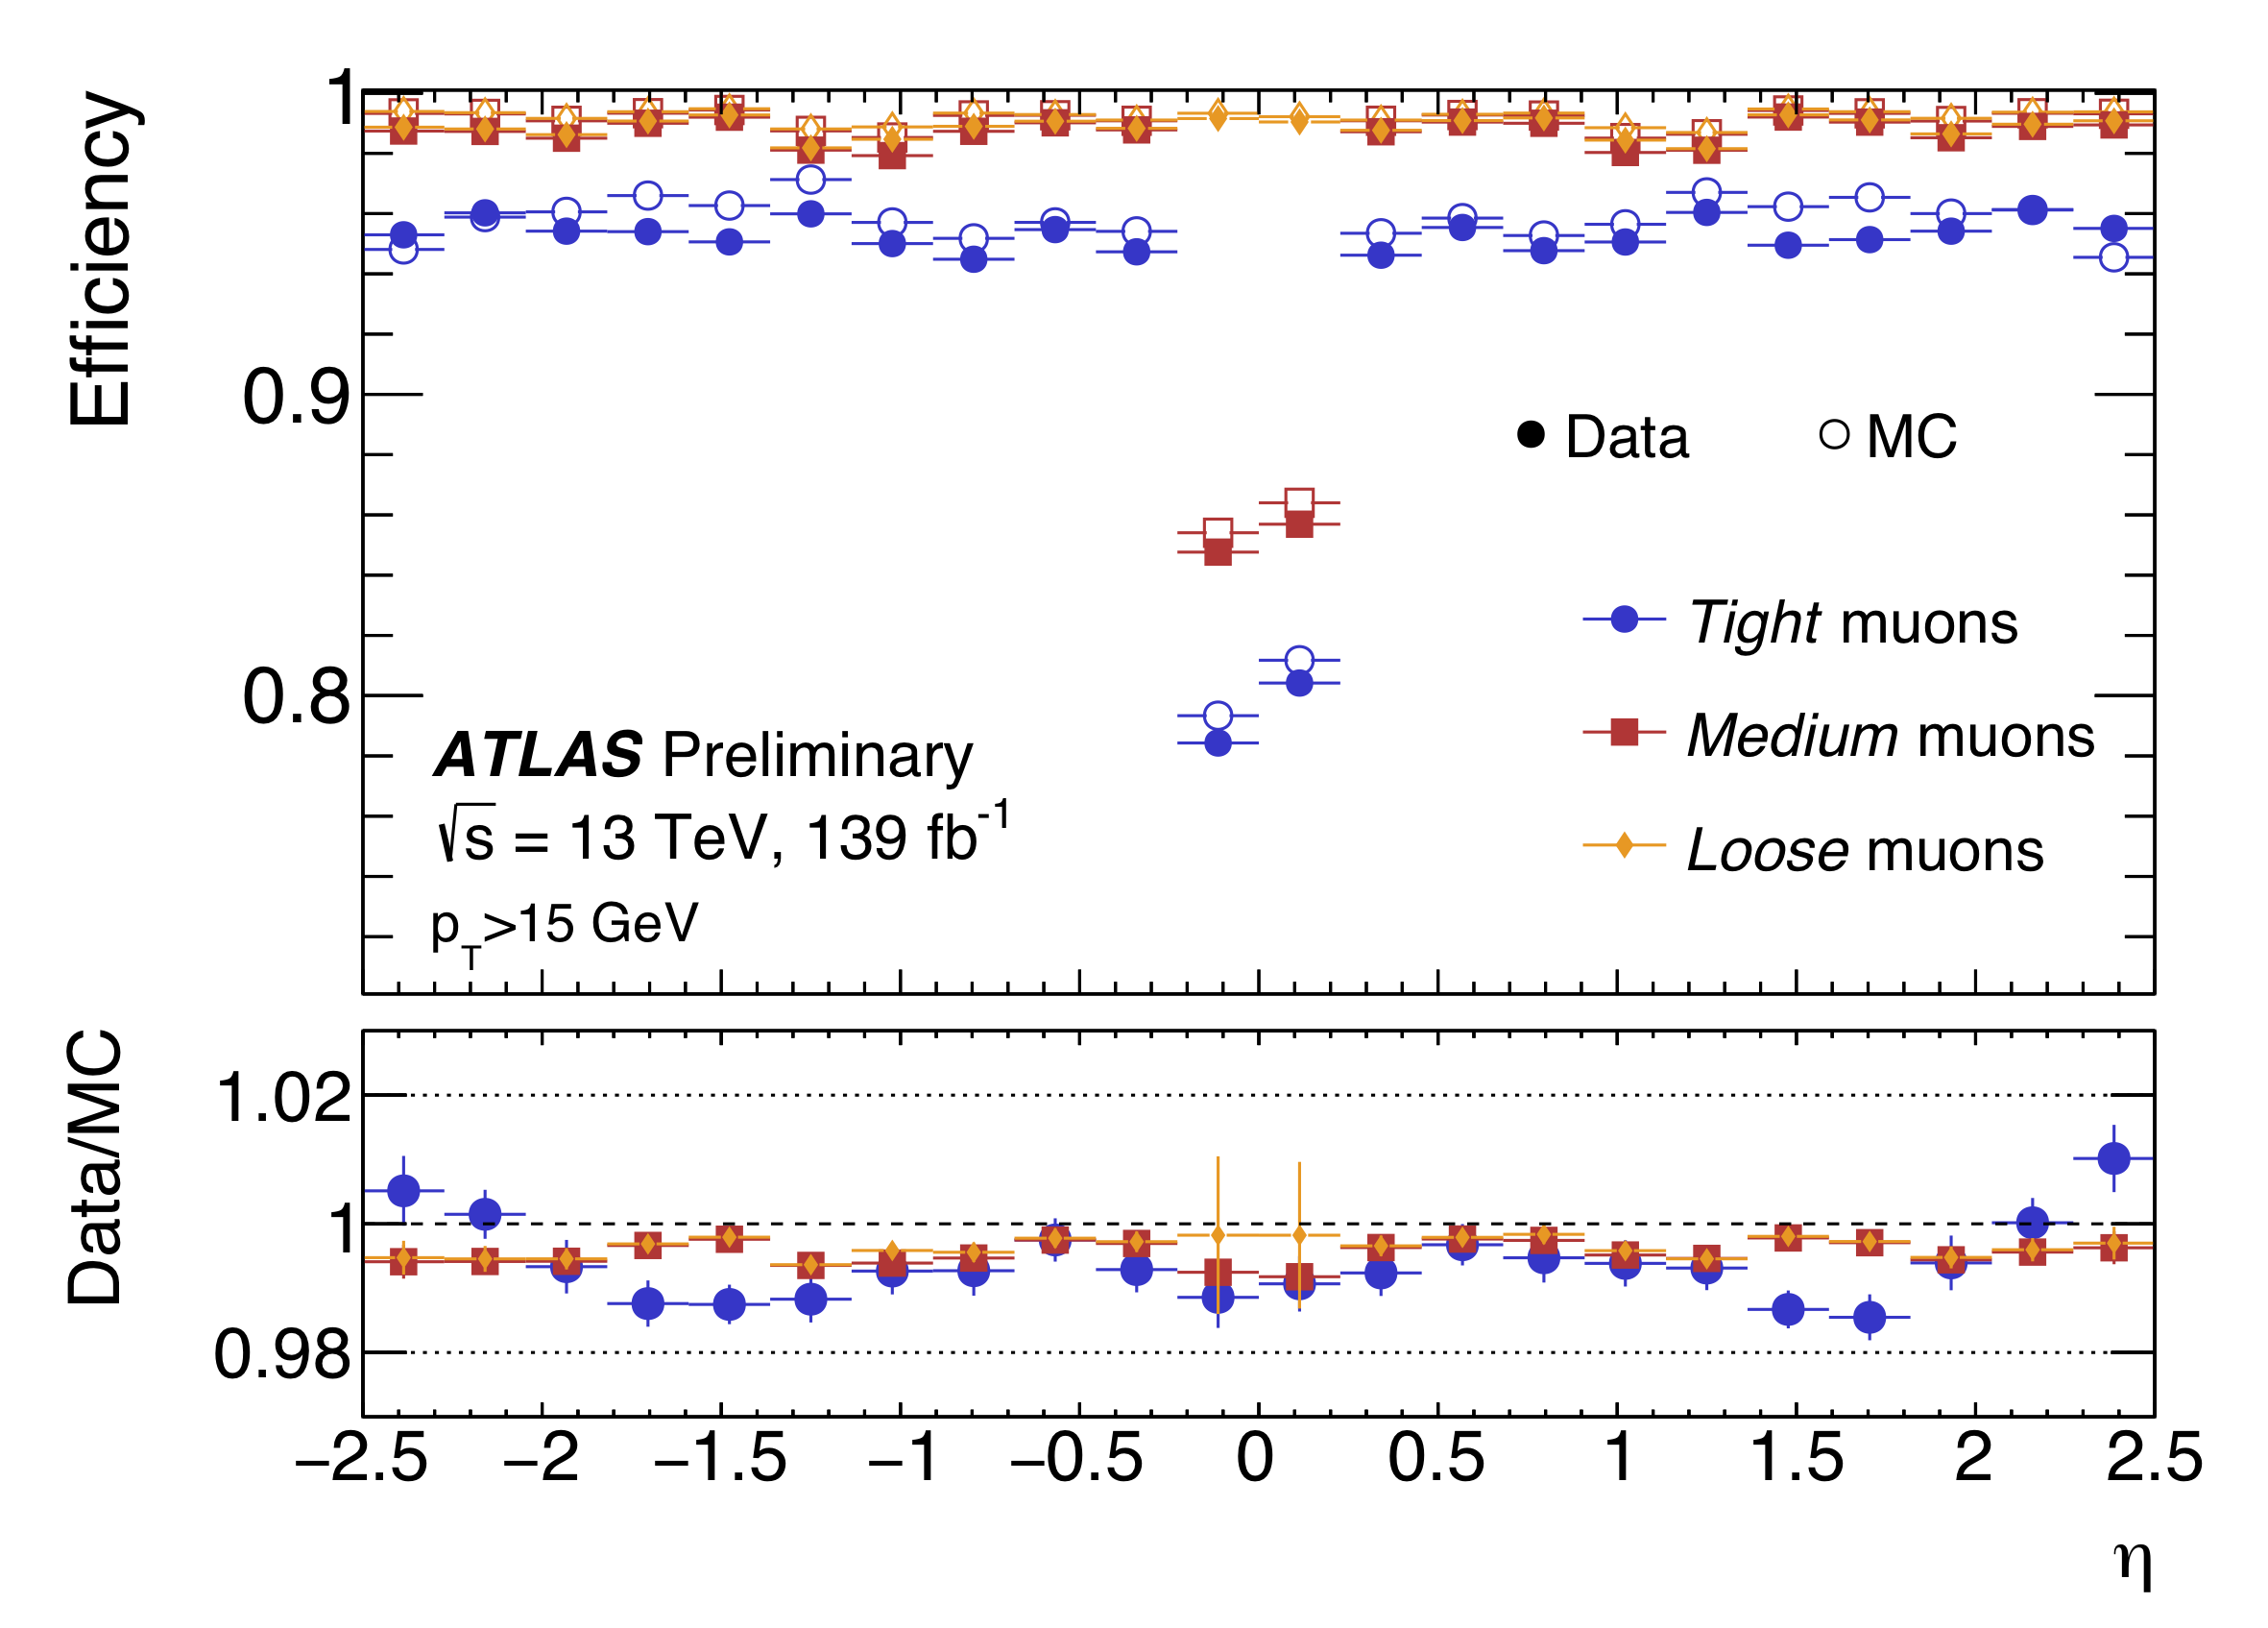
\includegraphics[width=0.8\textwidth]{figures/muons/reco_eff}
  \caption[Muon reconstruction efficiency.]{Muon reconstruction
  efficiency measurement for the Loose (yellow diamonds), Medium
  (red squares), and Tight (blue circles) selections in data
  (filled markers) and MC simulation (empty markers) as a function
  of muon pseudorapidity with $\pt > 15~\GeV$. The measurement
  uses $Z\rightarrow\mu\mu$ events in full Run 2 dataset of 139 $\ifb$
  at $\sqrt{s}=13~\TeV$. Error bars represent a quadratic sum of
  statistical and systematic uncertainties. From Ref. \cite{Junggeburth:2685295}}
  \label{fig:muon:reco_eff}
\end{figure}

\section{Momentum calibration}

Things that affect the resolution.

\section{Isolation}

\section{Isolation background subtraction}

\section{VADER4mu}

\section{Other objects}
